\ifx\wholebook\relax \else
% ------------------------ 

\documentclass{article}
%------------------- Other types of document example ------------------------
%
%\documentclass[twocolumn]{IEEEtran-new}
%\documentclass[12pt,twoside,draft]{IEEEtran}
%\documentstyle[9pt,twocolumn,technote,twoside]{IEEEtran}
%
%-----------------------------------------------------------------------------
%%
% loading packages
%
\newif\ifpdf
\ifx\pdfoutput\undefined % We're not running pdftex
  \pdffalse
\else
  \pdftrue
\fi
%
%
\ifpdf
  \RequirePackage[pdftex,%
            CJKbookmarks,%
       bookmarksnumbered,%
              colorlinks,%
          linkcolor=blue,%
              hyperindex,%
        plainpages=false,%
       pdfstartview=FitH]{hyperref}
\else
  \RequirePackage[dvipdfm,%
             CJKbookmarks,%
        bookmarksnumbered,%
               colorlinks,%
           linkcolor=blue,%
               hyperindex,%
         plainpages=false,%
        pdfstartview=FitH]{hyperref}
  \AtBeginDvi{\special{pdf:tounicode GBK-EUC-UCS2}} % GBK -> Unicode
\fi
\usepackage{hyperref}

% other packages
%-----------------------------------------------------------------------------
\usepackage{graphicx, color}
\usepackage{CJK}
%
% for programming 
%
\usepackage{verbatim}
\usepackage{listings}


\lstdefinelanguage{Smalltalk}{
  morekeywords={self,super,true,false,nil,thisContext}, % This is overkill
  morestring=[d]',
  morecomment=[s]{"}{"},
  alsoletter={\#:},
  escapechar={!},
  literate=
    {BANG}{!}1
    {UNDERSCORE}{\_}1
    {\\st}{Smalltalk}9 % convenience -- in case \st occurs in code
    % {'}{{\textquotesingle}}1 % replaced by upquote=true in \lstset
    {_}{{$\leftarrow$}}1
    {>>>}{{\sep}}1
    {^}{{$\uparrow$}}1
    {~}{{$\sim$}}1
    {-}{{\sf -\hspace{-0.13em}-}}1  % the goal is to make - the same width as +
    %{+}{\raisebox{0.08ex}{+}}1		% and to raise + off the baseline to match -
    {-->}{{\quad$\longrightarrow$\quad}}3
	, % Don't forget the comma at the end!
  tabsize=2
}[keywords,comments,strings]

\lstloadlanguages{C++, Lisp, Haskell, Python, Smalltalk}

% ======================================================================

\def\BibTeX{{\rm B\kern-.05em{\sc i\kern-.025em b}\kern-.08em
    T\kern-.1667em\lower.7ex\hbox{E}\kern-.125emX}}

\newtheorem{theorem}{Theorem}

%
% mathematics
%
\newcommand{\be}{\begin{equation}}
\newcommand{\ee}{\end{equation}}
\newcommand{\bmat}[1]{\left( \begin{array}{#1} }
\newcommand{\emat}{\end{array} \right) }
\newcommand{\VEC}[1]{\mbox{\boldmath $#1$}}

% numbered equation array
\newcommand{\bea}{\begin{eqnarray}}
\newcommand{\eea}{\end{eqnarray}}

% equation array not numbered
\newcommand{\bean}{\begin{eqnarray*}}
\newcommand{\eean}{\end{eqnarray*}}

\RequirePackage{CJK,CJKnumb,CJKulem,CJKpunct}
% we use CJK as default environment
\AtBeginDocument{\begin{CJK*}{GBK}{song}\CJKtilde\CJKindent\CJKcaption{GB}}
\AtEndDocument{\clearpage\end{CJK*}}

%
% loading packages
%

\RequirePackage{ifpdf}

%
%
\ifpdf
  \RequirePackage[pdftex,%
       bookmarksnumbered,%
              colorlinks,%
          linkcolor=blue,%
              hyperindex,%
        plainpages=false,%
       pdfstartview=FitH]{hyperref}
\else
  \RequirePackage[dvipdfm,%
        bookmarksnumbered,%
               colorlinks,%
           linkcolor=blue,%
               hyperindex,%
         plainpages=false,%
        pdfstartview=FitH]{hyperref}
\fi
\usepackage{hyperref}

% other packages
%--------------------------------------------------------------------------
\usepackage{graphicx, color}
\usepackage{subfig}

\usepackage{amsmath, amsthm, amssymb} % for math
\usepackage{exercise} % for exercise

%
% for programming 
%
\usepackage{verbatim}
\usepackage{listings}
%\usepackage{algorithmic} %old version; we can use algorithmicx instead
\usepackage{algorithm} 
\usepackage[noend]{algpseudocode} %for pseudo code, include algorithmicsx automatically
\usepackage{makeidx} % for index support


\lstdefinelanguage{Smalltalk}{
  morekeywords={self,super,true,false,nil,thisContext}, % This is overkill
  morestring=[d]',
  morecomment=[s]{"}{"},
  alsoletter={\#:},
  escapechar={!},
  literate=
    {BANG}{!}1
    {UNDERSCORE}{\_}1
    {\\st}{Smalltalk}9 % convenience -- in case \st occurs in code
    % {'}{{\textquotesingle}}1 % replaced by upquote=true in \lstset
    {_}{{$\leftarrow$}}1
    {>>>}{{\sep}}1
    {^}{{$\uparrow$}}1
    {~}{{$\sim$}}1
    {-}{{\sf -\hspace{-0.13em}-}}1  % the goal is to make - the same width as +
    %{+}{\raisebox{0.08ex}{+}}1		% and to raise + off the baseline to match -
    {-->}{{\quad$\longrightarrow$\quad}}3
	, % Don't forget the comma at the end!
  tabsize=2
}[keywords,comments,strings]

\lstloadlanguages{C++, Lisp, Haskell, Python, Smalltalk}

% ======================================================================

\def\BibTeX{{\rm B\kern-.05em{\sc i\kern-.025em b}\kern-.08em
    T\kern-.1667em\lower.7ex\hbox{E}\kern-.125emX}}

%
% mathematics
%
\newcommand{\be}{\begin{equation}}
\newcommand{\ee}{\end{equation}}
\newcommand{\bmat}[1]{\left( \begin{array}{#1} }
\newcommand{\emat}{\end{array} \right) }
\newcommand{\VEC}[1]{\mbox{\boldmath $#1$}}

% numbered equation array
\newcommand{\bea}{\begin{eqnarray}}
\newcommand{\eea}{\end{eqnarray}}

% equation array not numbered
\newcommand{\bean}{\begin{eqnarray*}}
\newcommand{\eean}{\end{eqnarray*}}

\newtheorem{theorem}{Theorem}[section]
\newtheorem{lemma}[theorem]{Lemma}
\newtheorem{proposition}[theorem]{Proposition}
\newtheorem{corollary}[theorem]{Corollary}


\setcounter{page}{1}

\begin{document}

\fi
%--------------------------

% ================================================================
%                 COVER PAGE
% ================================================================

\title{Queue, not so simple as it was thought}

\author{Liu~Xinyu
\thanks{{\bfseries Liu Xinyu } \newline
  Email: liuxinyu95@gmail.com \newline}
  }

\markboth{Queue}{AlgoXY}

\maketitle

\ifx\wholebook\relax
\chapter{Queue, not so simple as it was thought}
\numberwithin{Exercise}{chapter}
\fi

% ================================================================
%                 Introduction
% ================================================================
\section{Introduction}
\label{introduction}
It seems that queues are relative simple. A queue provides FIFO (first-in,
first-out) data manipulation support. There are many options to 
realize queue includes singly linked-list, doubly linked-list,
circular buffer etc. However, we'll show that it's not so easy to 
realize queue in purely functional settings if it must satisfy
abstract queue properties.

In this chapter, we'll present several different approaches to 
implement queue. And in next chapter, we'll explain how to realize
sequence.

A queue is a FIFO data structure satisfies the following performance
constraints.

\begin{itemize}
\item Element can be added to the tail of the queue in $O(1)$ constant time;
\item Element can be removed from the head of the queue in $O(1)$ constant time.
\end{itemize}

These two properties must be satisfied. And it's common to add some extra
goals, such as dynamic memory allocation etc.

Of course such abstract queue interface can be implemented with 
doubly-linked list trivially. But this is a overkill solution. 
We can even implement imperative queue with singly linked-list or
plain array. However, our main question here is about how to realize
a purely functional queue as well?

We'll first review the typical queue solution which is realized by
singly linked-list and circular buffer in first section; Then we
give a simple and straightforward functional solution in the second
section. While the performance is ensured in terms of amortized
constant time, we need find real-time solution (or worst-case solution)
for some special case. Such solution will be described in the third
and the fourth section. Finally, we'll show a very simple real-time
queue which depends on lazy evaluation.

Most of the functional contents are based on Chris, Okasaki's great
work in \cite{okasaki-book}. There are more than 16 different types
of purely functional queue given in that material.

% ================================================================
%                 Imperative queue
% ================================================================
\section{Queue by linked-list and circular buffer}

\subsection{Singly linked-list solution}
\index{Queue!Singly linked-list}

Queue can be implemented with singly linked-list. It's easy to add 
and remove element at the front end of a linked-list in $O(1)$ time. 
However, in
order to keep the FIFO order, if we execute one operation on head,
we must perform the inverse operation on tail.

For plain singly linked-list, we must traverse the whole list before
adding or removing. Traversing is bound to $O(N)$ time, 
where $N$ is the length of the list. This doesn't match the abstract
queue properties.

The solution is to use an extra record to store the tail of the linked-list.
A sentinel is often used to simplify the boundary handling. The 
following ANSI C \footnote{It's possible to parameterize the type of the key
with C++ template. ANSI C is used here for illustration purpose.} 
code defines a queue realized by singly linked-list.

\lstset{language=C}
\begin{lstlisting}
typedef int Key;

struct Node{
  Key key;
  struct Node* next;
};

struct Queue{
  struct Node *head, *tail;
};
\end{lstlisting}

Figure \ref{fig:empty-list} illustrates an empty list. Both head
and tail point to the sentinel NIL node.

\begin{figure}[htbp]
  \centering
  \includegraphics[scale=1.0]{img/empty-list.ps}
  \caption{The empty queue, both head and tail point to sentinel node.} \label{fig:empty-list}
\end{figure}

We summarize the abstract queue interface as the following.

\begin{algorithmic}
\Function{Empty}{}
  \Comment{Create an empty queue}
\EndFunction
\Function{Empty?}{$Q$}
  \Comment{Test if $Q$ is empty}
\EndFunction
\Function{Enqueue}{$Q, x$}
  \Comment{Add a new element $x$ to queue $Q$}
\EndFunction
\Function{Dequeue}{$Q$}
  \Comment{Remove element from queue $Q$}
\EndFunction
\Function{Head}{$Q$}
  \Comment{get the next element in queue $Q$ in FIFO order}
\EndFunction
\end{algorithmic}

Note the difference between \textproc{Dequeue} and \textproc{Head}.
\textproc{Head} only retrieve next element in FIFO order without removing
it, while \textproc{Dequeue} performs removing.

In some programming languages, such as Haskell, and most object-oriented
languages, the above abstract queue interface can be ensured by some definition.
For example, the following Haskell code specifies the abstract queue.

\lstset{language=Haskell}
\begin{lstlisting}
class Queue q where
    empty :: q a
    isEmpty :: q a -> Bool
    push :: q a -> a -> q a -- aka 'snoc' or append, or push_back
    pop :: q a -> q a -- aka 'tail' or pop_front
    front :: q a -> a -- aka 'head'
\end{lstlisting}

To ensure the constant time \textproc{Enqueue} and \textproc{Dequeue},
we add new element to head and remove element from tail.\footnote{It's possible
to add new element to the tail, while remove element from head, but the 
operations are more complex than this approach.}

\begin{algorithmic}
\Function{Enqueue}{$Q, x$}
  \State $p \gets $ \Call{Create-New-Node}{}
  \State \Call{Key}{$p$} $\gets x$
  \State \Call{Next}{$p$} $\gets NIL$
  \State \textproc{Next}(\Call{Tail}{$Q$}) $\gets p$
  \State \Call{Tail}{$Q$} $\gets p$
\EndFunction
\end{algorithmic}

Note that, as we use the sentinel node, there are at least one node, the
sentinel in the queue. That's why we needn't check the validation of
of the tail before we append the new created node $p$ to it.

\begin{algorithmic}
\Function{Dequeue}{$Q$}
  \State $x \gets $ \Call{Head}{$Q$}
  \State \textproc{Next}(\Call{Head}{$Q$}) $\gets$ \Call{Next}{$x$}
  \If{$x = $ \Call{Tail}{$Q$}} \Comment{$Q$ gets empty}
    \State \Call{Tail}{$Q$} $\gets$ \Call{Head}{$Q$}
  \EndIf
  \State \Return \Call{Key}{$x$}
\EndFunction
\end{algorithmic}

As we always put the sentinel node in front of all the other nodes,
function \textproc{Head} actually returns the next node to the sentinel.

Figure \ref{fig:list-queue} illustrates \textproc{Enqueue} and \textproc{Dequeue} process with sentinel node.

\begin{figure}[htbp]
 \centering
 \subfloat[Before \textproc{Enqueue} $x$ to queue]{\includegraphics[scale=0.8]{img/enq-list-before.ps}} \\
 \subfloat[After \textproc{Enqueue} $x$ to queue]{\includegraphics[scale=0.8]{img/enq-list-after.ps}} \\
 \subfloat[Before \textproc{Dequeue} $x$ to queue]{\includegraphics[scale=0.8]{img/deq-list-before.ps}} \\
 \subfloat[After \textproc{Dequeue} $x$ to queue]{\includegraphics[scale=0.8]{img/deq-list-after.ps}} \\
 \caption{\textproc{Enqueue} and \textproc{Dequeue} to linked-list queue.} \label{fig:list-queue}
\end{figure}

Translating the pseudo code to ANSI C program yields the below code.

\begin{lstlisting}
struct Queue* enqueue(struct Queue* q, Key x){
  struct Node* p = (struct Node*)malloc(sizeof(struct Node));
  p->key = x;
  p->next = NULL;
  q->tail->next = p;
  q->tail = p;
  return q;
}

Key dequeue(struct Queue* q){
  struct Node* p = head(q); /*gets the node next to sentinel*/
  Key x = key(p);
  q->head->next = p->next;
  if(q->tail == p)
    q->tail = q->head;
  free(p);
  return x;
}
\end{lstlisting}

This solution is simple and robust. It's easy to extend this solution 
even to the concurrent environment (e.g. multicores). We can assign
a lock to the head and use another lock to the tail. The sentinel 
helps us from being dead-locked due to the empty case \cite{PODC96} \cite{SutterDDJ}.

\begin{Exercise}
\begin{itemize}
\item Realize the \textproc{Empty?} and \textproc{Head} algorithms
for linked-list queue.

\item Implement the singly linked-list queue in your favorite imperative 
programming language. Note that you need provide functions to initialize
and destroy the queue.
\end{itemize}
\end{Exercise}

\subsection{Circular buffer solution}
\index{Queue!Circular buffer}

Another typical solution to realize queue is to use plain array as
a circular buffer (also known as ring buffer). 
Oppose to linked-list, array support appending to the 
tail in constant $O(1)$ time if there are still spaces. Of course
we need re-allocate spaces if the array is fully occupied. However,
Array performs poor in $O(N)$ time when removing element from head
and packing the space. This is because we need shift all rest elements
one cell ahead. The idea of circular buffer is to reuse the free
cells before the first valid element after we remove elements from
head.

The idea of circular buffer can be described in figure \ref{fig:circular-buffer-queue}
and \ref{fig:circular-buffer}.

\begin{figure}[htbp]
 \centering
 \subfloat[Continuously add some elements.]{\includegraphics[scale=0.8]{img/ring-buf-1.ps}} \\
 \subfloat[After remove some elements from head, there are free cells.]{\includegraphics[scale=0.8]{img/ring-buf-2.ps}} \\
 \subfloat[Go on adding elements till the boundary of the array.]{\includegraphics[scale=0.8]{img/ring-buf-3.ps}} \\
 \subfloat[The next element is added to the first free cell on head.]{\includegraphics[scale=0.8]{img/ring-buf-4.ps}} \\
 \subfloat[All cells are occupied. The queue is full.]{\includegraphics[scale=0.8]{img/ring-buf-5.ps}}
 \caption{A queue is realized with ring buffer.} \label{fig:circular-buffer-queue}
\end{figure}

\begin{figure}[htbp]
 \centering
 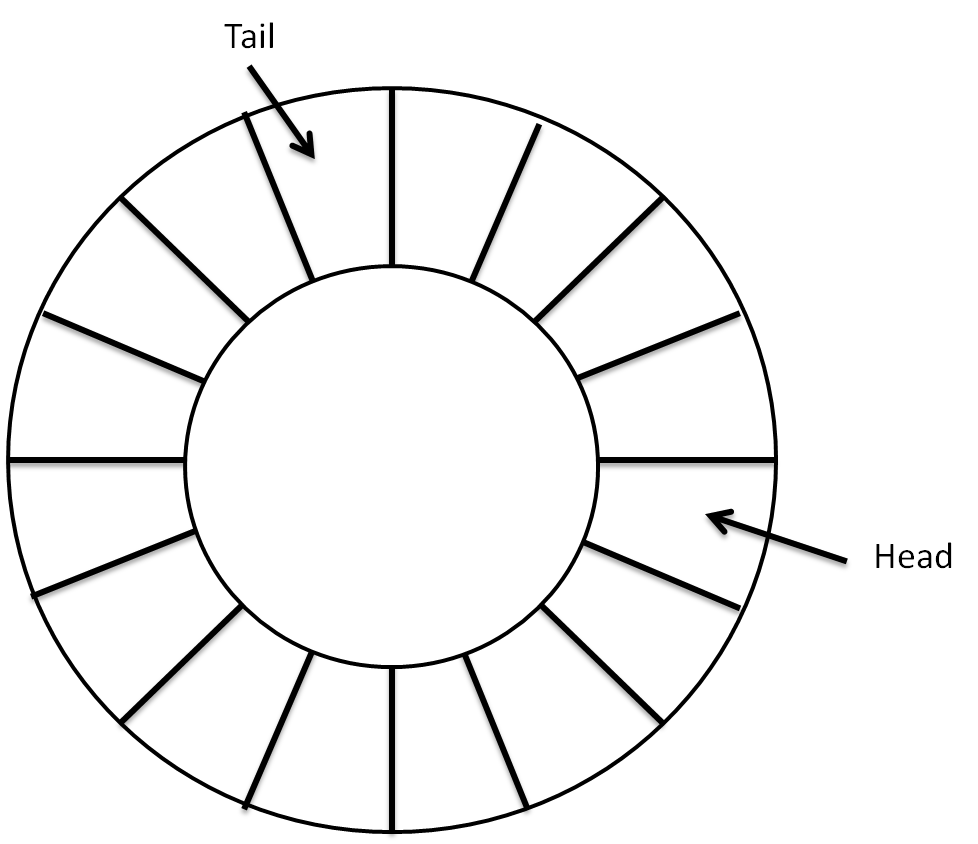
\includegraphics[scale=0.5]{img/ring-buffer.eps}
 \caption{The circular buffer.} \label{fig:circular-buffer}
\end{figure}

If we set a maximum size of the buffer instead of dynamically allocate 
memories, the queue can be defined with the below ANSI C code.

\lstset{language=C}
\begin{lstlisting}
struct Queue{
  Key* buf;
  int head, tail, size;
};
\end{lstlisting}

When initialize the queue, we are explicitly asked to provide the maximum
size as argument.

\begin{lstlisting}
struct Queue* createQ(int max){
  struct Queue* q = (struct Queue*)malloc(sizeof(struct Queue));
  q->buf = (Key*)malloc(sizeof(Key)*max);
  q->size = max;
  q->head = q->tail = 0;
  return q;
}
\end{lstlisting}

To test if a queue is empty is trivial.

\begin{algorithmic}
\Function{Empty?}{$Q$}
  \State \Return \Call{Head}{$Q$} = \Call{Tail}{$Q$}
\EndFunction
\end{algorithmic}

One brute-force implementation for \textproc{Enqueue} and \textproc{Dequeue}
is to calculate the modular of index blindly as the following.

\begin{algorithmic}
\Function{Enqueue}{$Q, x$}
  \If{$\lnot$ \Call{Full?}{$Q$}}
    \State \Call{Tail}{$Q$} $\gets $ (\Call{Tail}{$Q$} + 1) $\mod$ \Call{Size}{$Q$}
    \State \Call{Buffer}{$Q$}[\Call{Tail}{$Q$}] $\gets x$
  \EndIf
\EndFunction
\end{algorithmic}

\begin{algorithmic}
\Function{Head}{$Q$}
  \If{$\lnot$ \Call{Empty?}{$Q$}}
    \State \Return \Call{Buffer}{$Q$}[\Call{Head}{$Q$}]
  \EndIf
\EndFunction
\end{algorithmic}

\begin{algorithmic}
\Function{Dequeue}{$Q$}
  \If{$\lnot$ \Call{Empty?}{$Q$}}
    \State \Call{Head}{$Q$} $\gets $ (\Call{Head}{$Q$} + 1) $\mod$ \Call{Size}{$Q$}
  \EndIf
\EndFunction
\end{algorithmic}

However, modular is expensive and slow depends on some settings, so one
may replace it by some adjustment. For example as in the below ANSI C
program.

\begin{lstlisting}
void enQ(struct Queue* q, Key x){
  if(!fullQ(q)){
    q->buf[q->tail++] = x;
    q->tail -= q->tail< q->size ? 0 : q->size;
  }
}

Key headQ(struct Queue* q){
  return q->buf[q->head]; /* Assume queue isn't empty */
}

Key deQ(struct Queue* q){
  Key x = headQ(q);
  q->head++;
  q->head -= q->head< q->size ? 0 : q->size;
  return x;
}
\end{lstlisting}

\begin{Exercise}
As the circular buffer is allocated with a maximum size parameter, please
write a function to test if a queue is full to avoid overflow. Note
there are two cases, one is that the head is in front of the tail,
the other is on the contrary.
\end{Exercise}

% ================================================================
%                 the 1st version
% ================================================================
\section{Purely functional solution}

\subsection{Paired-list queue}
\index{Queue!Paired-list queue}

We can't just use a list to implement queue, or we can't satisfy abstract 
queue properties. This is because singly linked-list, which
is the back-end data structure in most functional settings, performs 
well on head in constant $O(1)$ time, while it performs in linear $O(N)$ 
time on tail, where $N$ is the length of the list. Either dequeue or enqueue
will perform proportion to the number of elements stored in the list
as shown in figure \ref{fig:linked-list-queue}.

\begin{figure}[htbp]
  \centering
  \subfloat[\textproc{DeQueue} performs poorly.]{\includegraphics[scale=0.5]{img/list-queue-head.ps}} \\
  \subfloat[\textproc{EnQueue} performs poorly.]{\includegraphics[scale=0.5]{img/list-queue-tail.ps}}
  \caption{\textproc{DeQueue} and \textproc{EnQueue} can't perform both in constant $O(1)$ time with a list.} \label{fig:linked-list-queue}
\end{figure}

We neither can add a pointer to record the tail position of the list
as what we have done in the imperative settings like in the ANSI C program,
because of the nature of purely functional.

Chris Okasaki mentioned a simple and straightforward functional solution
in \cite{okasaki-book}. The idea is to maintain two linked-lists as a queue, 
and concatenate these two lists in a tail-to-tail manner. The shape of the queue 
looks like a horseshoe magnet as shown in figure \ref{fig:horseshoe-magnet}.

\begin{figure}[htbp]
  \centering
  \subfloat[a horseshoe magnet.]{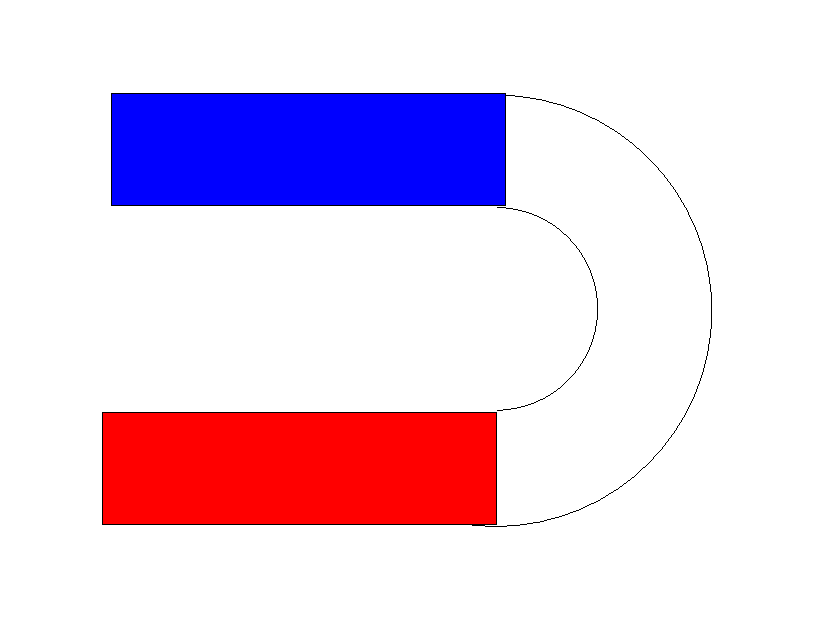
\includegraphics[scale=0.5]{img/horseshoe-magnet.eps}} \\
  \subfloat[concatenate two lists tail-to-tail.]{\includegraphics[scale=0.5]{img/front-rear-queue.ps}}
  \caption{A queue with front and rear list shapes like a horseshoe magnet.} \label{fig:horseshoe-magnet}
\end{figure}

With this setup, we push new element to the head of the rear list, which is
ensure to be $O(1)$ constant time; on the other hand, we pop element from
the head of the front list, which is also $O(1)$ constant time.
So that the abstract queue properties can be satisfied.

The definition of such paired-list queue can be expressed in the following
Haskell code.

\lstset{language=Haskell}
\begin{lstlisting}
type Queue a = ([a], [a])

empty = ([], [])
\end{lstlisting}

Suppose function $front(Q)$ and $rear(Q)$ return the front and rear
list in such setup, and $Queue(F, R)$ create a paired-list queue from
two lists $F$ and $R$.
The \textproc{EnQueue} (push) and \textproc{DeQueue} (pop) operations can
be easily realized based on this setup.

\be
push(Q, x) = Queue(front(Q), \{ x \} \cup rear(Q))
\ee

\be
pop(Q) = Queue(tail(front(Q)), rear(Q))
\ee

where if a list $X =  \{ x_1, x_2, ..., x_n \}$, 
function $tail(X) = \{ x_2, x_3, ..., x_n \}$ returns the rest of the list
without the first element.

However, we must next solve the problem that after several pop operations, 
the front
list becomes empty, while there are still elements in rear list. One method
is to rebuild the queue by reversing the rear list, and use it to replace front
list.

Hence a balance operation will be execute after popping. Let's denote the
front and rear list of a queue $Q$ as $F = front(Q)$, and $R = fear(Q)$.

\be
balance(F, R) = \left \{
  \begin{array}
  {r@{\quad:\quad}l}
  Queue(reverse(R), \Phi) & F = \Phi \\
  Q & otherwise 
  \end{array}
\right .
\ee

Thus if front list isn't empty, we do nothing, while when the front
list becomes empty, we use the reversed rear list as the new front list,
and the new rear list is empty.

The new enqueue and dequeue algorithms are updated as below.

\be
push(Q, x) = balance(F, \{ x \} \cup R)
\ee

\be
pop(Q) = balance(tail(F), R)
\ee

Sum up the above algorithms and translate them to Haskell yields the following
program.

\begin{lstlisting}
balance :: Queue a -> Queue a
balance ([], r) = (reverse r, [])
balance q = q

push :: Queue a -> a -> Queue a
push (f, r) x = balance (f, x:r)

pop :: Queue a -> Queue a
pop ([], _) = error "Empty"
pop (_:f, r) =  balance (f, r)
\end{lstlisting}

However, although we only touch the heads of front list and rear list, the 
overall performance can't be kept always as $O(1)$. Actually, the performance
of this algorithm is amortized $O(1)$. This is because the reverse operation
takes time proportion to the length of the rear list. it's bound $O(N)$
time, where $N = |R|$. We left the prove of amortized performance as 
an exercise to the reader.

\subsection{Paired-array queue - a symmetric implementation}
\index{Queue!Paired-array queue}

There is an interesting implementation which is symmetric to the paired-list
queue. In some old programming languages, such as legacy version of BASIC,
There is array supported, but there is no pointers, nor records to represent
linked-list. Although we can use another array to store indexes so that we
can represent linked-list with implicit array, there is another option to
realized amortized $O(1)$ queue.

Compare the performance of array and linked-list. Below table reveals some
facts (Suppose both contain $N$ elements).

\begin{tabular}{l | c | r}
  \hline
  operation & Array & Linked-list \\
  \hline
  insert on head & $O(N)$ & $O(1)$ \\
  insert on tail & $O(1)$ & $O(N)$ \\
  remove on head & $O(N)$ & $O(1)$ \\
  remove on tail & $O(1)$ & $O(N)$ \\
  \hline
\end{tabular}

Note that linked-list performs in constant time on head, but in linear time on tail;
while array performs in constant time on tail (suppose there is enough memory spaces, and
omit the memory reallocation for simplification), but in linear time on head.
This is because we need do shifting when prepare or eliminate an empty cell in array.
(see chapter 'the evolution of insertion sort' for detail.)

The above table shows an interesting characteristic, that we can exploit it and provide
a solution mimic to the paired-list queue: We concatenate two arrays, head-to-head, to
make a horseshoe shape queue like in figure \ref{fig:horseshoe-array}.

\begin{figure}[htbp]
  \centering
  \subfloat[a horseshoe magnet.]{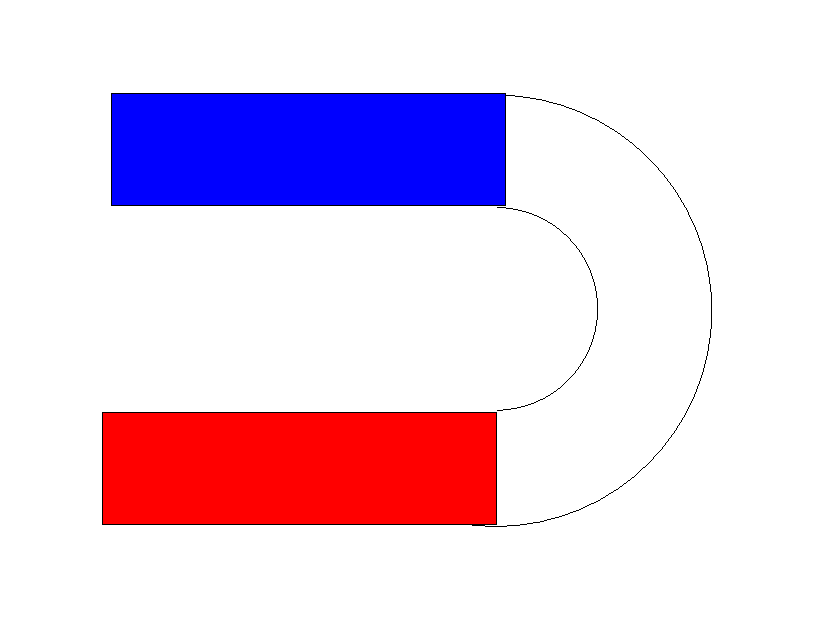
\includegraphics[scale=0.5]{img/horseshoe-magnet.eps}}
  \subfloat[concatenate two arrays head-to-head.]{\includegraphics[scale=0.5]{img/front-rear-array-queue.ps}}
  \caption{A queue with front and rear arrays shapes like a horseshoe magnet.} \label{fig:horseshoe-array}
\end{figure}

We can define such paired-array queue like the following Python code \footnote{Legacy Basic
code is not presented here. And we actually use list but not array in Python to illustrate the idea.
ANSI C and ISO C++ programs are provides along with this chapter, they show more
in a purely array manner.}

\lstset{language=Python}
\begin{lstlisting}
class Queue:
    def __init__(self):
        self.front = []
        self.rear = []

def is_empty(q):
    return q.front == [] and q.rear == []
\end{lstlisting}

The relative \textproc{Push}() and \textproc{Pop}() algorithm only manipulate
on the tail of the arrays.

\begin{algorithmic}
\Function{Push}{$Q, x$}
  \State \textproc{Append}(\Call{Rear}{$Q$}, $x$)
\EndFunction
\end{algorithmic}

Here we assume that the \textproc{Append}() algorithm append element $x$ to
the end of the array, and handle the necessary memory allocation etc. Actually,
there are multiple memory handling approaches. For example, besides the 
dynamic re-allocation, we can initialize the array with enough space, and just 
report error if it's full.

\begin{algorithmic}
\Function{Pop}{$Q$}
  \If{\Call{Front}{$Q$} $= \Phi$}
    \State \Call{Front}{$Q$} $\gets$ \textproc{Reverse}(\Call{Rear}{$Q$})
    \State \Call{Rear}{$Q$} $\gets \Phi$ 
  \EndIf
  \State $N \gets$ \textproc{Length}(\Call{Front}{$Q$})
  \State $x \gets$ \Call{Front}{$Q$}[N]
  \State \textproc{Length}(\Call{Front}{$Q$}) $\gets N - 1$
  \State \Return $x$
\EndFunction
\end{algorithmic}

For simplification and pure illustration purpose, the array isn't shrunk
explicitly after elements removed. So test if front array is empty ($\Phi$)
can be realized as check if the length of the array is zero. We omit all
these details here.

The enqueue and dequeue algorithms can be translated to Python programs
straightforwardly.

\begin{lstlisting}
def push(q, x):
    q.rear.append(x)

def pop(q):
    if q.front == []:
        q.rear.reverse()
        (q.front, q.rear) = (q.rear, [])
    return q.front.pop()
\end{lstlisting}

Similar to the paired-list queue, the performance is amortized $O(1)$
because the reverse procedure takes linear time.

\begin{Exercise}
\begin{itemize}
\item Prove that the amortized performance of paired-list queue is $O(1)$.
\item Prove that the amortized performance of paired-array queue is $O(1)$.
\end{itemize}
\end{Exercise}

% ================================================================
%                 Balanced Queue
% ================================================================
\section{A small improvement, Balanced Queue}
\index{Queue!Balance Queue}

Although paired-list queue is amortized $O(1)$ for popping and pushing,
the solution we proposed in previous section performs poor in the worst case.
For example, there is one element in the front list, and we push $N$ elements
continuously to the queue, here $N$ is a big number. After that executing
a pop operation will cause the worst case.

According to the strategy we used so far, all the $N$ elements are added
to the rear list. The front list turns to be empty after a pop operation.
So the algorithm starts to reverse the rear list. This reversing procedure
is bound to $O(N)$ time, which is proportion to the length of the rear
list. Sometimes, it can't be
acceptable for a very big $N$.

The reason why this worst case happens is because the front and rear lists
are extremely unbalanced. We can improve our paired-list queue design
by making them more balanced. One option is to add a balancing constraint.

\be
  | R | \leq | F |
\label{eq:balance-invariant}
\ee

Where $R = Rear(Q)$, $F = Front(Q)$, and $|L|$ is the length of list $L$. 
This constraint ensure the length
of the rear list is less than the length of the front list. So that the reverse
procedure will be executed once the rear list grows longer than
the front list.

Here we need frequently access the length information of a list. However,
calculate the length takes linear time for singly linked-list. We can 
record the length to a variable and update it as adding and removing elements.
This approach enables us to get the length information in constant time.

Below example shows the modified paired-list queue definition which is augmented 
with length fields.

\lstset{language=Haskell}
\begin{lstlisting}
data BalanceQueue a = BQ [a] Int [a] Int
\end{lstlisting}

As we keep the invariant as specified in (\ref{eq:balance-invariant}), we
can easily tell if a queue is empty by testing the length of the front list.

\be
  F = \Phi \Leftrightarrow |F| = 0
\ee

In the rest part of this section, we suppose the length of a list $L$, can
be retrieved as $|L|$ in constant time.

Push and pop are almost as same as before except that we check the balance
invariant by passing length information and performs reversing accordingly.

\be
  push(Q, x) = balance(F, |F|, \{ x \} \cup R, |R| + 1)
\ee

\be
  pop(Q) = balance(tail(F), |F|-1, R, |R|)
\ee

Where function $balance()$ is defined as the following.

\be
  balance(F, |F|, R, |R|) = \left \{
  \begin{array}
  {r@{\quad:\quad}l}
  Queue(F, |F|, R, |R|) & |R| \leq |F| \\
  Queue(F \cup reverse(R), |F| + |R|, \Phi, 0) & otherwise 
  \end{array}
\right .
\ee

Note that the function $Queue()$ takes four parameters, the front list along
with its length (recorded), and the rear list along with its length, and
forms a paired-list queue augmented with length fields.

We can easily translate the equations to Haskell program. And we can
enforce the abstract queue interface by making the implementation
an instance of the Queue type class.

\lstset{language=Haskell}
\begin{lstlisting}
instance Queue BalanceQueue where
    empty = BQ [] 0 [] 0

    isEmpty (BQ _ lenf _ _) = lenf == 0

    -- Amortized O(1) time push
    push (BQ f lenf r lenr) x = balance f lenf (x:r) (lenr + 1)

    -- Amortized O(1) time pop
    pop (BQ (_:f) lenf r lenr) = balance f (lenf - 1) r lenr

    front (BQ (x:_) _ _ _) = x

balance f lenf r lenr
    | lenr <= lenf = BQ f lenf r lenr
    | otherwise = BQ (f ++ (reverse r)) (lenf + lenr) [] 0
\end{lstlisting}

\begin{Exercise}
Write the symmetric balance improvement solution for paired-array queue
in your favorite imperative programming language.
\end{Exercise}

% ================================================================
%                 Realtime Queue
% ================================================================
\section{One more step improvement, Real-time Queue}
\index{Queue!Real-time Queue}

Although the extremely worst case can be avoided by improving the balancing
as what has been presented in previous section, the performance 
of reversing rear list is still bound to $O(N)$, where $N = |R|$.
So if the rear list is very long, the instant performance is still
unacceptable poor even if the amortized time is $O(1)$. It is particularly
important in some real-time system to ensure the worst case performance.

As we have analyzed, the bottleneck is the computation of $ F \cup reverse(R)$.
This happens when $|R| > |F|$. Considering that $|F|$ and $|R|$ are
all integers, so this computation happens when

\be
  |R| = |F| + 1
\ee

Both $F$ and the result of $reverse(R)$ are singly linked-list, 
It takes $O(|F|)$ time to concatenate them together, and it takes extra
$O(|R|)$ time to reverse the rear list, so the total computation
is bound to $O(|N|)$, where $N = |F| + |R|$. Which is proportion to the 
total number of elements in the queue.

In order to realize a real-time queue, we can't computing $ F \cup reverse(R)$
monolithic. Our strategy is to distribute this expensive computation to every
pop and push operations. Thus although each pop and push get a bit slow,
we may avoid the extremely slow worst pop or push case.

\subsubsection{Incremental reverse}
\index{Queue!Incremental reverse}

Let's examine how functional reverse algorithm is implemented typically.

\be
  reverse(X) = \left \{
  \begin{array}
  {r@{\quad:\quad}l}
  \Phi & X = \Phi \\
  reverse(X') \cup \{ x_1 \} & otherwise
  \end{array}
\right .
\ee

Where $X' = tail(X) = \{ x_2, x_3, ...\}$.

This is a typical recursive algorithm, that if the list to be reversed is
empty, the result is just an empty list. This is the edge case; otherwise, we 
take the first element $x_1$ from the list, reverse the rest $\{x_2, x_3, ..., x_n \}$, 
to $\{x_n, x_{n-1}, .., x_3, x_2 \}$ and append $x_1$ after it.

However, this algorithm performs poor, as appending an element to the end of a list
is proportion to the length of the list. So it's $O(N^2)$, but not a linear
time reverse algorithm.

There exists another implementation which utilizes an accumulator $A$, like below.

\be
  reverse(X) = reverse'(X, \Phi)
\ee

Where

\be
 reverse'(X, A) = \left \{
  \begin{array}
  {r@{\quad:\quad}l}
  A & X = \Phi \\
  reverse'(X', \{ x_1 \} \cup A) & otherwise
  \end{array}
\right .
\ee

We call $A$ as {\em accumulator} because it accumulates intermediate reverse result
at any time. Every time we call $reverse'(X, A)$, list $X$ contains the rest of
elements wait to be reversed, and $A$ holds all the reversed elements so far. For instance
when we call $reverse'()$ at $i$-th time, $X$ and $A$ contains the following
elements:

\[
  \begin{array}{r@{\quad}l}
  X = \{x_i, x_{i+1}, ..., x_n \} & A = \{ x_{i-1}, x_{i-2}, ... x_1 \}
  \end{array}
\]

In every non-trivial case, we takes the first element from $X$ in $O(1)$ time;
then put it in front of the accumulator $A$, which is again $O(1)$ constant time.
We repeat it $N$ times, so this is a linear time ($O(N)$) algorithm.

The latter version of reverse is obviously a {\em tail-recursion} algorithm,
see \cite{tail-call} and \cite {recursion} for detail. Such characteristic 
is easy to change from monolithic algorithm to incremental manner.

The solution is state transferring. We can use a state machine contains
two types of stat: reversing state $S_r$ to indicate that the reverse
is still on-going (not finished), and finish state $S_f$ to indicate
the reverse has been done (finished). In Haskell programming
language, it can be defined as a type.

\lstset{language=Haskell}
\begin{lstlisting}
data State a = | Reverse [a] [a]
               | Done [a]
\end{lstlisting}

And we can schedule (slow-down) the above $reverse'(X, A)$ function with
these two types of state.

\be
  step(S, X, A) = \left \{
  \begin{array}
  {r@{\quad:\quad}l}
  (S_f, A) & S = S_r \land X = \Phi \\
  (S_r, X', \{ x_1 \} \cup A) & S = S_r \land X \neq \Phi \\
  \end{array}
\right .
\ee

Each step, we examine the state type first, if the current state is
$S_r$ (on-going), and the rest elements to be reversed in $X$ is
empty, we can turn the algorithm to finish state $S_f$; otherwise,
we take the first element from $X$, put it in front of $A$ just
as same as above, but we do NOT perform recursion, instead, we 
just finish this
step. We can store the current state as well as the resulted $X$ 
and $A$, the reverse can be continued at any time when we call 'next' 
$step$ function in the future with the stored state, $X$ and $A$ 
passed in.

Here is an example of this step-by-step reverse algorithm.

\[
\begin{array}{lcl}
step(S_r, "hello", \Phi) & = & (S_r, "ello", "h") \\
step(S_r, "ello", "h") & = & (S_r, "llo", "eh") \\
... & & \\
step(S_r, "o", "lleh") & = & (S_r, \Phi, "olleh") \\
step(S_r, \Phi, "olleh") & = & (S_f, "olleh")
\end{array}
\]

And in Haskell code manner, the example is like the following.

\lstset{language=Haskell}
\begin{lstlisting}
step $ Reverse "hello" [] = Reverse "ello" "h"
step $ Reverse "ello" "h" = Reverse "llo" "eh"
...
step $ Reverse "o" "lleh" = Reverse [] "olleh"
step $ Reverse [] "olleh" = Done "olleh"
\end{lstlisting}

Now we can distribute the reverse into steps in every pop and push 
operations. However, the problem is just half solved. We want to
break down $ F \cup reverse(R)$, and we have broken $reverse(R)$
into steps, we next need to schedule(slow-down) the list concatenation
part $F \cup ...$, which is bound to $O(|F|)$, into incremental
manner so that we can distribute it to pop and push operations.

\subsubsection{Incremental concatenate}
\index{Queue!Incremental concatenate}

It's a bit more challenge to implement incremental list concatenation
than list reversing. However, it's possible to re-use the result
we gained from increment reverse by a small trick: In order to 
realize $X \cup Y$, we can first reverse $X$ to $\overleftarrow{X}$,
then take elements one by one from $\overleftarrow{X}$ and put
them in front of $Y$ just as what we have done in $reverse'$.

\be
  \begin{array}{rcl}
    X \cup Y & \equiv & reverse(reverse(X)) \cup Y \\
             & \equiv & reverse'(reverse(X), \Phi) \cup Y \\
             & \equiv & reverse'(reverse(X), Y) \\
             & \equiv & reverse'(\overleftarrow{X}, Y)
  \end{array}
\ee

This fact indicates us that we can use an extra state to instruct
the $step()$ function to continuously concatenating $\overleftarrow{F}$
after $R$ is reversed.

The strategy is to do the total work in two phases:
\begin{enumerate}
\item Reverse both $F$ and $R$ in parallel to get $\overleftarrow{F} = reverse(F)$, and 
$\overleftarrow{R} = reverse(R)$ incrementally;
\item Incrementally take elements from $\overleftarrow{F}$ and put them in front of
$\overleftarrow{R}$.
\end{enumerate}

So we define three types of state: $S_r$ represents reversing; $S_c$ represents
concatenating; and $S_f$ represents finish.

In Haskell, these types of state are defined as the following.

\lstset{language=Haskell}
\begin{lstlisting}
data State a = Reverse [a] [a] [a] [a]
             | Concat [a] [a]
             | Done [a]
\end{lstlisting}

Because we reverse $F$ and $R$ simultaneously, so reversing state takes two
pairs of lists and accumulators.

The state transfering is defined according to the two phases strategy described
previously.
Denotes that $F = \{ f_1, f_2, ... \}$, $F' = tail(F) = \{f_2, f_3, ... \}$,
$R = \{ r_1, r_2, ... \}$, $R' = tail(R) = \{ r_2, r_3, ... \}$. A state $\mathcal{S}$,
contains it's type $S$, which has the value among $S_r$, $S_c$, and $S_f$. 
Note that $\mathcal{S}$ also contains necessary 
parameters such as $F$, $\overleftarrow{F}$, $X$, $A$ etc as intermediate results.
These parameters vary according to the different states.

\be
  next(\mathcal{S}) = \left \{
  \begin{array}
  {r@{\quad:\quad}l}
  (S_r, F', \{ f_1 \} \cup \overleftarrow{F}, R', \{ r_1 \} \cup \overleftarrow{R}) & S = S_r \land F \neq \Phi \land R \neq \Phi \\
  (S_c, \overleftarrow{F}, \{ r_1 \} \cup \overleftarrow{R}) & S = S_r \land F = \Phi \land R = \{ r_1 \} \\
  (S_f, A) & S = S_c \land X = \Phi \\
  (S_c, X', \{ x_1 \} \cup A) & S = S_c \land X \neq \Phi
  \end{array}
\right .
\ee

The relative Haskell program is list as below.

\lstset{language=Haskell}
\begin{lstlisting}
next (Reverse (x:f) f' (y:r) r') = Reverse f (x:f') r (y:r')
next (Reverse [] f' [y] r') = Concat f' (y:r')
next (Concat 0 _ acc) = Done acc
next (Concat (x:f') acc) = Concat f' (x:acc)
\end{lstlisting}

All left to us is to distribute these incremental steps into every pop and push
operations to implement a real-time $O(1)$ purely functional queue.

\subsubsection{Sum up}

Before we dive into the final real-time queue implementation. Let's analyze how
many incremental steps are taken to achieve the result of $F \cup reverse(R)$.
According to the balance variant we used previously, $|R| = |F| + 1$, Let's 
denotes $M = |F|$. 

Once the queue gets unbalanced due to some push or pop operation, we start this
incremental  $F \cup reverse(R)$.
It needs $M + 1$ steps to reverse $R$, and at the same time, we finish reversing
the list $F$ within these steps. After that, we need extra $M+1$ steps to execute
the concatenation. So there are $2M + 2$ steps.

It seems that distribute one step inside one pop or push operation is the natural
solution, However, there is a critical 
question must be answered: Is it possible that before we finish these $2M + 2$ steps,
the queue gets unbalanced again due to a series push and pop?

There are two facts about this question, one is good news and the other is bad news.

Let's first show the good news, that luckily, continuously pushing can't make the 
queue unbalanced again before we finish these $2M + 2$ steps to achieve $F \cup reverse(R)$.
This is because once we start re-balancing, we can get a new front list 
$F' = F \cup reverse(R)$ after $2M + 2$ steps. While the next time unbalance
is triggered when 

\be
  \begin{array}{rcl}
  |R'| & = & |F'| + 1 \\
       & = & |F| + |R| + 1 \\
       & = & 2M + 2
  \end{array}
\ee

That is to say, even we continuously pushing as mush elements as possible after 
the last unbalanced time, when the queue gets unbalanced again, the $2M+2$ steps
exactly get finished at that time point. Which means the new front list $F'$ is
calculated OK. We can safely go on to compute $F' \cup reverse(R')$. Thanks to the
balance invariant which is designed in previous section.

But, the bad news is that, pop operation can happen at anytime before these
$2M+2$ steps finish. The situation is that once we want to extract element 
from front list, the new front list $F' = F \cup reverse(R)$ hasn't been
ready yet. We don't have a valid front list at hand.

One solution to solve this problem is to keep a copy of original front list $F$,
during the time we are calculating $reverse(F)$ which is described in phase 1 of
our incremental computing strategy. So that we are still safe even if user
continuously performs first $M$ pop operations. So the queue looks like
in table \ref{tab:pop-before-m} at some time after we start the incremental computation and before
phase 1 (reverse $F$ and $R$ simultaneously) ending.

\begin{table}
\centering
\begin{tabular}{l l l}
  front copy & on-going computation & new rear \\
  \hline
  $\{ f_i, f_{i+1}, ..., f_M \}$ & $(S_r, \tilde{F}, ..., \tilde{R}, ...)$ & $ \{ ... \}$ \\
  first $i-1$ elements popped & intermediate result $\overleftarrow{F}$ and $\overleftarrow{R}$ & new elements pushed
\end{tabular}
\caption{Intermediate state of a queue before first $M$ steps finish.}
\label{tab:pop-before-m}
\end{table}

After these $M$ pop operations, the copy of $F$ is exhausted. And we just
start incremental concatenation phase at that time. What if user goes
on popping?

The fact is that since $F$ is exhausted (becomes $\Phi$), we needn't do concatenation
at all. Since $F \cup \overleftarrow{R} = \Phi \cup \overleftarrow{R} = \overleftarrow{R}$.

It indicates us, when doing concatenation, we only need to concatenate those elements
haven't been popped, which are still left in $F$. As user pops elements one by one
continuously from the head of front list $F$, one method is to use a counter,
record how many elements there are still in $F$. The counter is initialized as 0
when we start computing $F \cup reverse(R)$, it's increased by one when we reverse
one element in $F$, which means we need concatenate thie element in the future; 
and it's decreased by one every time when pop is
performed, which means we can concatenate one element less; of course we need decrease
this counter as well in every steps of concatenation. If and only if this counter
becomes zero, we needn't do concatenations any more.

We can give the realization of purely functional real-time queue according to the above
analysis.

We first add an idle state $S_0$ to simplify some state transfering. Below Haskell program
is an example of this modified state definition.

\lstset{language=Haskell}
\begin{lstlisting}
data State a = Empty
             | Reverse Int [a] [a] [a] [a] -- n, f', acc_f' r, acc_r
             | Append Int [a] [a]          -- n, rev_f', acc
             | Done [a] -- result: f ++ reverse r
\end{lstlisting}

And the data structure is defined with three parts, the front list (augmented with length);
the on-going state of computing $F \cup reverse(R)$; and the rear list (augmented with length).

Here is the Haskell definition of real-time queue.

\lstset{language=Haskell}
\begin{lstlisting}
data RealtimeQueue a = RTQ [a] Int (State a) [a] Int
\end{lstlisting}

The empty queue is composed with empty front and rear list together with idle state $S_0$ as
$Queue(\Phi, 0, S_0, \Phi, 0)$. And we can test if a queue is empty by checking if $|F| = 0$ 
according
to the balance invariant defined before. Push and pop are changed accordingly.

\be
  push(Q, x) = balance(F, |F|, \mathcal{S}, \{ x \} \cup R, |R|+1)
\ee

\be
  pop(Q) = balance(F', |F|-1, abort(\mathcal{S}), R, |R|)
\ee

The major difference is $abort()$ function. Based on our above analysis, when there
is popping, we need decrease the counter, so that we can concatenate one element less.
We define this as aborting. The details will be given after $balance()$ function.

The relative Haskell code for push and pop are listed like this.

\lstset{language=Haskell}
\begin{lstlisting}
push (RTQ f lenf s r lenr) x = balance f lenf s (x:r) (lenr + 1)
pop (RTQ (_:f) lenf s r lenr) = balance f (lenf - 1) (abort s) r lenr
\end{lstlisting}

The $balance()$ function first check the balance invariant, if it's violated, we need
start re-balance it by starting compute $F \cup reverse(R)$ incrementally; otherwise
we just execute one step of the unfinished incremental computation. 

\be
  balance(F, |F|, \mathcal{S}, R, |R|) = \left \{
  \begin{array}
  {r@{\quad:\quad}l}
  step(F, |F|, \mathcal{S}, R, |R|) & |R| \leq |F| \\
  step(F, |F| + |R|, (S_r, 0, F, \Phi, R, \Phi) \Phi, 0) & otherwise
  \end{array}
\right .
\ee

The relative Haskell code is given like below.

\lstset{language=Haskell}
\begin{lstlisting}
balance f lenf s r lenr 
    | lenr <= lenf =  step f lenf s r lenr
    | otherwise = step f (lenf + lenr) (Reverse 0 f [] r []) [] 0
\end{lstlisting}

The $step()$ function typically transfer the state machine one state ahead, and
it will turn the state to idle ($S_0$) when the incremental computation finishes.

\be
  step(F, |F|, \mathcal{S}, R, |R|) = \left \{
  \begin{array}
  {r@{\quad:\quad}l}
  Queue(F', |F|, S_0, R, |R|) &  S' = S_f \\
  Queue(F, |F|, \mathcal{S}', R, |R|) & otherwise
  \end{array}
  \right .
\ee

Where $\mathcal{S}' = next(\mathcal{S})$ is the next state transferred; 
$F' = F \cup reverse(R)$, is the final new front list result from the incremental
computing. The real
state transferring is implemented in $next()$ function as the following. It's different
from previous version by adding the counter field $n$ to record how many elements left
we need to concatenate.

\be
  next(\mathcal{S}) = \left \{
  \begin{array}
  {r@{\quad:\quad}l}
  (S_r, n+1, F', \{ f_1 \} \cup \overleftarrow{F}, R', \{ r_1 \} \cup \overleftarrow{R}) &
      S = S_r \land F \neq \Phi \\
  (S_c, n, \overleftarrow{F}, \{ r_1 \} \cup \overleftarrow{R}) &
      S = S_r \land F = \Phi \\
  (S_f, A) & S = S_c \land n = 0 \\
  (S_c, n-1, X', \{ x_1 \} \cup A) & S = S_c \land n \neq 0 \\
  \mathcal{S} & otherwise
  \end{array}
\right .
\ee

And the corresponding Haskell code is like this.

\lstset{language=Haskell}
\begin{lstlisting}
next (Reverse n (x:f) f' (y:r) r') = Reverse (n+1) f (x:f') r (y:r')
next (Reverse n [] f' [y] r') = Concat n f' (y:r')
next (Concat 0 _ acc) = Done acc
next (Concat n (x:f') acc) = Concat (n-1) f' (x:acc)
next s = s
\end{lstlisting}

Function $abort()$ is used to tell the state machine, we can concatenate one element
less since it is popped.

\be
  abort(\mathcal{S}) = \left \{
  \begin{array}
  {r@{\quad:\quad}l}
  (S_f, A') & S = S_c \land n = 0 \\
  (S_c, n-1, X' A) & S = S_c \land n \neq 0 \\
  (S_r, n-1, F, \overleftarrow{F}, R, \overleftarrow{R}) & S = S_r \\
  \mathcal{S} & otherwise
  \end{array}
\right .
\ee

Note that when $n = 0$ we actually rollback one concatenated element by 
return $A'$ as the result but not $A$. (Why? this is left as an exercise.)

The Haskell code for abort function is like the following.

\lstset{language=Haskell}
\begin{lstlisting}
abort (Concat 0 _ (_:acc)) = Done acc -- Note! we rollback 1 elem
abort (Concat n f' acc) = Concat (n-1) f' acc
abort (Reverse n f f' r r') = Reverse (n-1) f f' r r'
abort s = s
\end{lstlisting}

It seems that we've done, however, there is still one tricky issue hidden 
behind us.
If we push an element $x$ to an empty queue, the result queue will be:
\[
  Queue(\Phi, 1, (S_c, 0, \Phi, \{ x \}), \Phi, 0)
\]

If we perform pop immediately, we'll get an error! We found that  
the front list is empty although the previous computation of $F \cup reverse(R)$ 
has been finished. This is because it takes one more extra step to
transfer from the state $(S_c, 0, \Phi, A)$ to $(S_f, A)$. It's necessary
to refine the $\mathcal{S}'$ in $step()$ function a bit.

\be
  \mathcal{S}' = \left \{
  \begin{array}
  {r@{\quad:\quad}l}
  next(next(\mathcal{S})) & F = \Phi \\
  next(\mathcal{S}) & otherwise
  \end{array}
\right .
\ee

The modification reflects to the below Haskell code:

\lstset{language=Haskell}
\begin{lstlisting}
step f lenf s r lenr =
    case s' of 
      Done f' -> RTQ f' lenf Empty r lenr
      s' -> RTQ f lenf s' r lenr
    where s' = if null f then next $ next s else next s
\end{lstlisting} %$

Note that this algorithm differs from the one given by Chris Okasaki in \cite{okasaki-book}.
Okasaki's algorithm executes two steps per pop and push, while the one presents in 
this chapter executes only one per pop and push, which leads to more distributed
performance.

\begin{Exercise}
\begin{itemize}
\item Why need we rollback one element when $n=0$ in $abort()$ function?

\item Realize the real-time queue with symmetric paired-array queue solution in your favorite 
imperative programming language.
\end{itemize}
\end{Exercise}


% ================================================================
%                 Lazy Real-time queue
% ================================================================
\section{Lazy real-time queue}
\index{Queue!Lazy real-time queue}

The key to realize a real-time queue is to break down the expensive
$F \cup reverse(R)$ to avoid monolithic computation. Lazy evaluation
is particularly helpful in such case. In this section, we'll explore
if there is some more elegant solution by exploit laziness.

Suppose that there exits a function $rotate()$,
which can compute $F \cup reverse(R)$ incrementally. that's to say,
with some accumulator $A$, the following two functions are equivalent.

\be
  rotate(X, Y, A) \equiv X \cup reverse(Y) \cup A
  \label{eq:rot-def}
\ee

Where we initialized $X$ as the front list $F$, $Y$ as the rear list $R$,
and the accumulator $A$ is initialized as empty $\Phi$.

The trigger of rotation is still as same as before when $|F| + 1 = |R|$.
Let's keep this constraint as an invariant during the whole rotation process,
that $|X| + 1 = |Y|$ always holds.

It's obvious to deduce to the trivial case:

\be
  rotate(\Phi, \{ y_1 \}, A) = \{ y_1 \} \cup A
\ee

Denote $X = \{ x_1, x_2, ... \}$, $Y = \{ y_1, y_2, ...\}$, and
$X' = \{ x_2, x_3, ...  \}$, $Y' = \{ y_2, y_3, ...\}$ are the rest
of the lists without the first element for $X$ and $Y$ respectively.
The recursion case is ruled out as the following.

\be
  \begin{array}{rcll}
  rotate( X, Y, A ) & \equiv & X \cup reverse(Y) \cup A & \mbox{Definition of (}\ref{eq:rot-def} \mbox{)} \\
  & \equiv & \{ x_1 \} \cup (X' \cup reverse(Y) \cup A) & \mbox{Associative of } \cup \\
  & \equiv & \{ x_1 \} \cup (X' \cup reverse(Y') \cup (\{ y_1 \} \cup A)) & \mbox{Nature of reverse and associative of }  \cup \\
  & \equiv & \{ x_1 \} \cup rotate(X', Y', \{ y_1 \} \cup A) & \mbox{Definition of (} \ref{eq:rot-def} \mbox{)}
  \end{array}
\ee

Summarize the above two cases, yields the final incremental rotate algorithm.

\be
rotate(X, Y, A) = \left \{
  \begin{array}
  {r@{\quad:\quad}l}
  \{ y_1 \} \cup A & X = \Phi \\
  \{ x_1 \} \cup rotate(X', Y', \{ y_1 \} \cup A) & otherwise
  \end{array}
\right .
\ee

If we execute $\cup$ lazily instead of strictly, that is, execute $\cup$
once pop or push operation is performed, the computation of $rotate$ can
be distribute to push and pop naturally.

Based on this idea, we modify the paired-list queue definition to change
the front list to a lazy list, and augment it with a computation stream.
\cite{SICP}. When the queue triggers re-balance constraint by some
pop/push, that
$|F| + 1 = |R|$, The algorithm creates a lazy rotation computation,
then use this lazy rotation as the new front list $F'$; the new rear
list becomes $\Phi$, and a copy of $F'$ is maintained as a stream.

After that, when we performs every push and pop; we consume the 
stream by forcing a $\cup$ operation. This results us advancing one
step along the stream, $ \{ x \} \cup F''$, where $F' = tail(F')$.
We can discard $x$, and replace the stream $F'$ with $F''$.

Once all of the stream is exhausted, we can start another rotation.

In order to illustrate this idea clearly, we turns to Scheme/Lisp
programming language to show example codes, because it gives us
explicit control of laziness.

In Scheme/Lisp, we have the following three tools to deal with lazy
stream.

\lstset{language=Lisp}
\begin{lstlisting}
(define (cons-stream a b) (cons a (delay b)))

(define stream-car car)

(define (stream-cdr s) (cdr (force s)))
\end{lstlisting}

So 'cons-stream' constructs a 'lazy' list from an element $x$
and an existing list $L$ without really evaluating
the value of $L$; The evaluation is actually delayed to 
'stream-cdr', where the computation is forced. delaying can 
be realized by lambda calculus, please refer to \cite{SICP} for
detail.

The lazy paired-list queue is defined as the following.

\lstset{language=Lisp}
\begin{lstlisting}
(define (make-queue f r s)
  (list f r s))

;; Auxiliary functions
(define (front-lst q) (car q))

(define (rear-lst q) (cadr q))

(define (rots q) (caddr q))
\end{lstlisting}

A queue is consist of three parts, a front list, a rear list,
and a stream which represents the computation of $F \cup reverse(R)$.
Create an empty queue is trivial as making all these three parts
null.

\begin{lstlisting}
(define empty (make-queue '() '() '()))
\end{lstlisting}

Note that the front-list is also lazy stream actually, so we need use
stream related functions to manipulate it. For example, the following
function test if the queue is empty by checking the front lazy list stream.

\begin{lstlisting}
(define (empty? q) (stream-null? (front-lst q)))
\end{lstlisting}

The push function is almost as same as the one given in previous section.
That we put the new element in front of the rear list; and then examine
the balance invariant and do necessary balancing works.

\be
push(Q, x) = balance(\mathcal{F}, \{ x \} \cup R, \mathcal{R}_s)
\ee

Where $\mathcal{R}$ represents the lazy stream of front list; $\mathcal{R}_s$ is 
the stream of rotation computation. The relative Scheme/Lisp
code is give below.

\begin{lstlisting}
(define (push q x)
  (balance (front-lst q) (cons x (rear q)) (rots q)))
\end{lstlisting}

While pop is a bit different, because the front list is actually lazy stream,
we need force an evaluation. All the others are as same as before.

\be
pop(Q) = balance(\mathcal{F}', R, \mathcal{R}_s)
\ee

Here $\mathcal{F}'$, force one evaluation to $\mathcal{F}$, the Scheme/Lisp
code regarding to this equation is as the following. 

\begin{lstlisting}
(define (pop q)
  (balance (stream-cdr (front-lst q)) (rear q) (rots q)))
\end{lstlisting}

For illustration purpose, we skip the error handling (such as pop from
an empty queue etc) here.

And one can access the top element in the queue by extract from 
the front list stream.

\begin{lstlisting}
(define (front q) (stream-car (front-lst q)))
\end{lstlisting}

The balance function first checks if the computation stream is completely
exhausted, and starts new rotation accordingly; otherwise, it just consumes
one evaluation by enforcing the lazy stream.

\be
balance(Q) = \left \{
  \begin{array}
  {r@{\quad:\quad}l}
  Queue(\mathcal{F}', \Phi, \mathcal{F}') & \mathcal{R}_s = \Phi \\
  Queue(\mathcal{F}, R, \mathcal{R}_s') & otherwise
  \end{array}
\right .
\ee

Here $\mathcal{F}'$ is defined to start a new rotation.

\be
  \mathcal{F}' = rotate(F, R, \Phi)
\ee

The relative Scheme/Lisp program is listed accordingly.

\begin{lstlisting}
(define (balance f r s)
  (if (stream-null? s)
      (let ((newf (rotate f r '())))
    (make-queue newf '() newf))
      (make-queue f r (stream-cdr s))))
\end{lstlisting}

The implementation of incremental rotate function is just as same as
what we analyzed above.

\begin{lstlisting}
(define (rotate xs ys acc)
  (if (stream-null? xs)
      (cons-stream (car ys) acc)
      (cons-stream (stream-car xs)
           (rotate (stream-cdr xs) (cdr ys)
               (cons-stream (car ys) acc)))))
\end{lstlisting}

We used explicit lazy evaluation in Scheme/Lisp. Actually, this program
can be very short by using lazy programming languages, for example,
Haskell.

\lstset{language=Haskell}
\begin{lstlisting}
data LazyRTQueue a = LQ [a] [a] [a] -- front, rear, f ++ reverse r

instance Queue LazyRTQueue where
    empty = LQ [] [] []

    isEmpty (LQ f _ _) = null f

    -- O(1) time push
    push (LQ f r rot) x = balance f (x:r) rot

    -- O(1) time pop
    pop (LQ (_:f) r rot) = balance f r rot

    front (LQ (x:_) _ _) = x

balance f r [] = let f' = rotate f r [] in LQ f' [] f'
balance f r (_:rot) = LQ f r rot

rotate [] [y] acc = y:acc
rotate (x:xs) (y:ys) acc = x : rotate xs ys (y:acc)
\end{lstlisting}

% ================================================================
%                 Short summary
% ================================================================
\section{Notes and short summary}
Just as mentioned in the beginning of this book in the first chapter,
queue isn't so simple as it was thought. We've tries to explain 
algorithms and data structures both in imperative and in function 
approaches; Sometimes, it gives impression that functional way is
simpler and more expressive in most time. However, there are still
plenty of areas, that more studies and works are needed to give equivalent
functional solution. Queue is such an important topic, that it
links to many fundamental purely functional data structures.

That's why Chris Okasaki made intensively study and took a great
amount of discussions in \cite{okasaki-book}. With purely functional
queue solved, we can easily implement dequeue with the similar
approach revealed in this chapter. As we can handle elements effectively
in both head and tail, we can advance one step ahead to realize
sequence data structures, which support fast concatenate, and
finally we can realize random access data structures to mimic
array in imperative settings. The details will be explained
in later chapters.

Note that, although we haven't mentioned priority queue, it's quite 
possible to realized it with heaps. We have covered topic of heaps
in several previous chapters.

\begin{Exercise}
\begin{itemize}
\item Realize dequeue, wich support adding and removing elements on both sides in
constant $O(1)$ time in purely functional way.
\item Realize dequeue in a symmetric solution only with array in your
favorite imperative programming language.
\end{itemize}
\end{Exercise}

% ================================================================
%                 Appendix
% ================================================================

\begin{thebibliography}{99}

\bibitem{PODC96}
Maged M. Michael and Michael L. Scott. ``Simple, Fast, and Practical Non-Blocking and Blocking Concurrent Queue Algorithms''. http://www.cs.rochester.edu/research/synchronization/pseudocode/queues.html

\bibitem{SutterDDJ}
Herb Sutter. ``Writing a Generalized Concurrent Queue''. Dr. Dobb's Oct 29, 2008. http://drdobbs.com/cpp/211601363?pgno=1

\bibitem{CLRS}
Thomas H. Cormen, Charles E. Leiserson, Ronald L. Rivest and Clifford Stein. ``Introduction to Algorithms, Second Edition''. The MIT Press, 2001. ISBN: 0262032937.

\bibitem{okasaki-book}
Chris Okasaki. ``Purely Functional Data Structures''. Cambridge university press, (July 1, 1999), ISBN-13: 978-0521663502

\bibitem{tail-call}
Wikipedia. ``Tail-call''. http://en.wikipedia.org/wiki/Tail\_call

\bibitem{recursion}
Wikipedia. ``Recursion (computer science)''. http://en.wikipedia.org/wiki/Recursion\_(computer\_science)\#Tail-recursive\_functions

\bibitem{SICP}
Harold Abelson, Gerald Jay Sussman, Julie Sussman. ``Structure and Interpretation of Computer Programs, 2nd Edition''. MIT Press, 1996, ISBN 0-262-51087-1

\end{thebibliography}

\ifx\wholebook\relax \else
\end{document}
\fi
